\documentclass[tikz,border=2pt]{standalone}
\usepackage{tikz}
\usepackage{helvet}
\renewcommand{\familydefault}{\sfdefault}
\usetikzlibrary{arrows.meta, positioning, fit, backgrounds, shapes.geometric, calc}

% ---- band colors: exact viridis(5) sampling used in Fig. 7 / Fig. 4 of the paper ----
\definecolor{bandA}{HTML}{440154} % Low-freq (Trend)
\definecolor{bandB}{HTML}{3B528B} % Mid-low (Cycle)
\definecolor{bandC}{HTML}{21918C} % Mid (Seasonal)
\definecolor{bandD}{HTML}{5EC962} % Mid-high (Short-term)
\definecolor{bandE}{HTML}{FDE725} % High-freq (Noise)

\definecolor{inputgrey}{HTML}{4A4A4A}
\definecolor{panelbg}{HTML}{F5F5F5}
\definecolor{panelline}{HTML}{9A9A9A}
\definecolor{fusionblue}{HTML}{2E5EAA}

\begin{document}
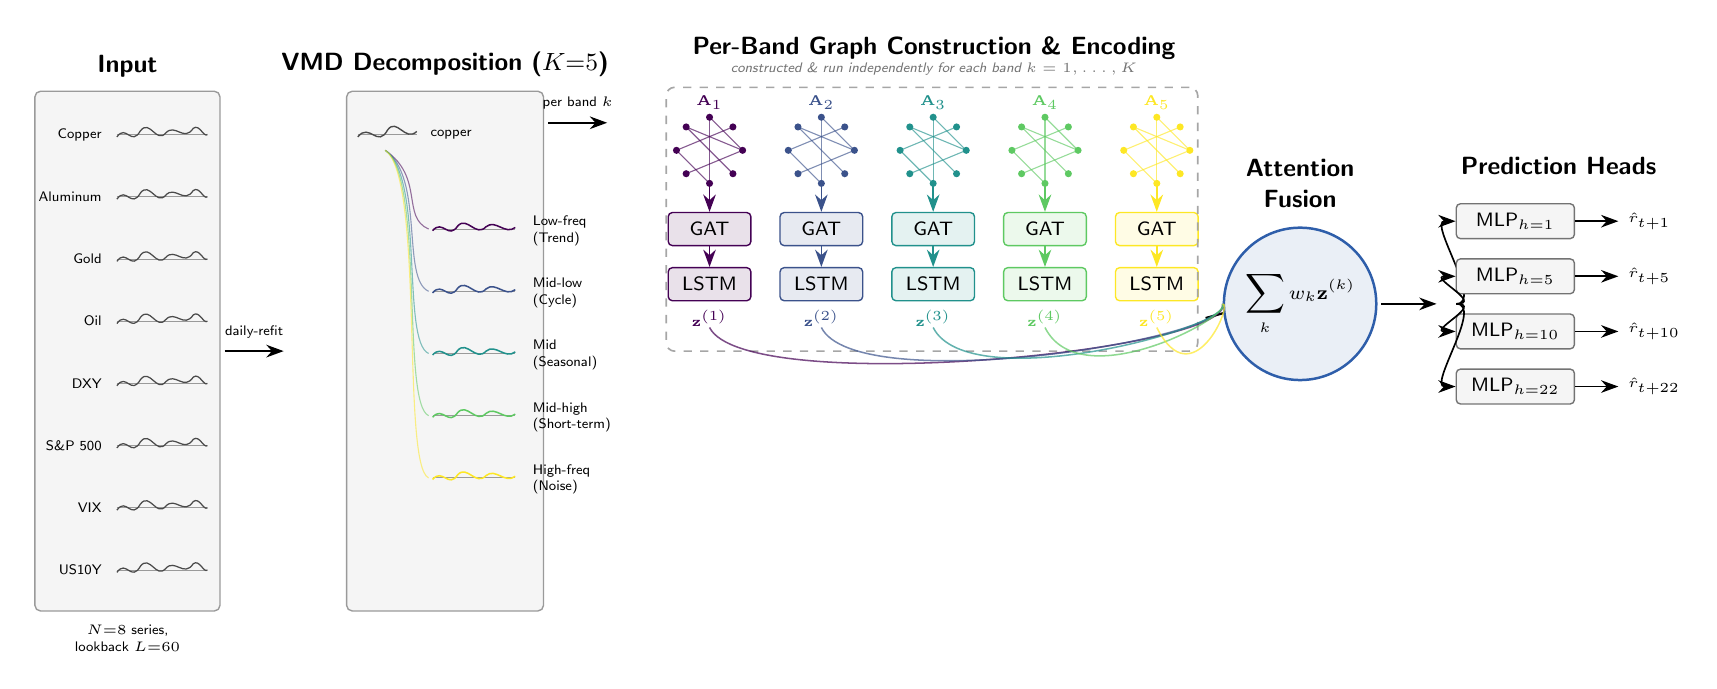
\begin{tikzpicture}[
    font=\sffamily\footnotesize,
    >={Stealth[length=2.2mm,width=1.6mm]},
    every node/.style={align=center},
    panel/.style={draw=panelline, rounded corners=2pt, fill=panelbg, line width=0.5pt},
    modblock/.style={draw=black!55, rounded corners=1.5pt, fill=white, minimum width=1.05cm, minimum height=0.42cm, font=\sffamily\scriptsize, line width=0.5pt},
    groupbox/.style={draw=black!35, dashed, rounded corners=3pt, line width=0.6pt},
]

% ============================================================
% COLUMN 1: raw multivariate input
% ============================================================
\node[panel, minimum width=2.35cm, minimum height=6.6cm] (inputpanel) at (0,0) {};
\node[above=0.05cm of inputpanel.north, font=\sffamily\bfseries\small] {Input};

\foreach \i/\lbl in {0/Copper, 1/Aluminum, 2/Gold, 3/Oil, 4/DXY, 5/S\&P 500, 6/VIX, 7/US10Y} {
    \pgfmathsetmacro{\yy}{2.75 - \i*0.79}
    \node[anchor=east, font=\sffamily\tiny] at ($(inputpanel.west) + (0.98,\yy)$) {\lbl};
    \begin{scope}[shift={($(inputpanel.west) + (1.05,\yy)$)}]
        \draw[panelline, line width=0.3pt] (0,0) -- (1.15,0);
        \draw[inputgrey, line width=0.45pt]
            (0,-0.03) .. controls (0.12,0.14) and (0.18,-0.16) .. (0.30,0.05)
            .. controls (0.42,0.20) and (0.50,-0.12) .. (0.62,0.02)
            .. controls (0.74,0.15) and (0.85,-0.10) .. (0.97,0.08)
            .. controls (1.05,0.14) and (1.10,-0.04) .. (1.15,0.00);
    \end{scope}
}
\node[below=0.05cm of inputpanel.south, font=\sffamily\tiny, text width=2.3cm] {$N{=}8$ series, lookback $L{=}60$};

% ============================================================
% ARROW 1
% ============================================================
\draw[->, line width=0.8pt] ($(inputpanel.east)+(0.05,0)$) -- ++(0.75,0)
    node[midway, above, font=\sffamily\tiny, yshift=1pt] {daily-refit};

% ============================================================
% COLUMN 2: VMD decomposition -- copper trace fanning into K=5 bands
% ============================================================
\coordinate (vmdanchor) at ($(inputpanel.east)+(1.6,0)$);
\node[panel, minimum width=2.5cm, minimum height=6.6cm] (vmdpanel) at ($(vmdanchor)+(1.25,0)$) {};
\node[above=0.05cm of vmdpanel.north, font=\sffamily\bfseries\small] {VMD Decomposition ($K{=}5$)};

% source trace (copper)
\begin{scope}[shift={($(vmdpanel.west)+(0.15,2.75)$)}]
    \draw[panelline, line width=0.3pt] (0,0) -- (0.75,0);
    \draw[inputgrey, line width=0.5pt]
        (0,-0.03) .. controls (0.15,0.16) and (0.25,-0.18) .. (0.38,0.06)
        .. controls (0.50,0.22) and (0.60,-0.10) .. (0.75,0.04);
\end{scope}
\node[anchor=west, font=\sffamily\tiny] at ($(vmdpanel.west)+(0.95,2.75)$) {copper};

% fan lines from source to 5 bands
\foreach \i/\col/\lblone/\lbltwo in {%
    0/bandA/Low-freq/(Trend),%
    1/bandB/Mid-low/(Cycle),%
    2/bandC/Mid/(Seasonal),%
    3/bandD/Mid-high/(Short-term),%
    4/bandE/High-freq/(Noise)%
} {
    \pgfmathsetmacro{\yy}{1.55 - \i*0.79}
    \draw[\col, line width=0.4pt, opacity=0.55]
        ($(vmdpanel.west)+(0.5,2.55)$) .. controls ($(vmdpanel.west)+(1.0,2.2)$) and ($(vmdpanel.west)+(0.7,\yy+0.15)$) .. ($(vmdpanel.west)+(1.05,\yy)$);
    \begin{scope}[shift={($(vmdpanel.west)+(1.1,\yy)$)}]
        \draw[panelline, line width=0.3pt] (0,0) -- (1.05,0);
        \draw[\col, line width=0.55pt]
            (0,-0.02) .. controls (0.13,0.13) and (0.20,-0.14) .. (0.32,0.04)
            .. controls (0.44,0.17) and (0.55,-0.11) .. (0.68,0.03)
            .. controls (0.80,0.13) and (0.92,-0.08) .. (1.05,0.02);
    \end{scope}
    \node[anchor=west, font=\sffamily\tiny, text width=1.1cm, align=left] at ($(vmdpanel.west)+(2.25,\yy-0.02)$) {\lblone\\\lbltwo};
}

% ============================================================
% ARROW 2
% ============================================================
\draw[->, line width=0.8pt] ($(vmdpanel.east)+(0.05,2.9)$) -- ++(0.75,0)
    node[midway, above, font=\sffamily\tiny, yshift=1pt] {per band $k$};

% ============================================================
% COLUMN 3: per-band graph construction + GAT + LSTM  (the central claim)
% ============================================================
\coordinate (bandcolstart) at ($(vmdpanel.east)+(1.55,0)$);

% helper macro: an 8-node circular graph icon, colored, with a handful of illustrative edges
\newcommand{\graphicon}[2]{%
    % #1 = color, #2 = radius
    \begin{scope}
        \foreach \a in {0,45,...,315} {
            \coordinate (gn-\a) at (\a:#2);
        }
        \draw[#1, line width=0.4pt, opacity=0.65] (gn-0) -- (gn-90);
        \draw[#1, line width=0.4pt, opacity=0.65] (gn-0) -- (gn-135);
        \draw[#1, line width=0.4pt, opacity=0.65] (gn-45) -- (gn-180);
        \draw[#1, line width=0.4pt, opacity=0.65] (gn-90) -- (gn-270);
        \draw[#1, line width=0.4pt, opacity=0.65] (gn-135) -- (gn-315);
        \draw[#1, line width=0.4pt, opacity=0.65] (gn-180) -- (gn-270);
        \draw[#1, line width=0.4pt, opacity=0.65] (gn-225) -- (gn-0);
        \foreach \a in {0,45,...,315} {
            \fill[#1] (gn-\a) circle (0.045);
        }
    \end{scope}
}

\node[font=\sffamily\bfseries\small] at ($(bandcolstart)+(3.4,3.85)$) {Per-Band Graph Construction \& Encoding};
\node[font=\sffamily\tiny\itshape, black!55] at ($(bandcolstart)+(3.4,3.58)$) {constructed \& run independently for each band $k=1,\ldots,K$};

\foreach \i/\col in {0/bandA, 1/bandB, 2/bandC, 3/bandD, 4/bandE} {
    \pgfmathsetmacro{\xx}{\i*1.42}
    \pgfmathtruncatemacro{\kk}{\i+1}

    % graph icon
    \begin{scope}[shift={($(bandcolstart)+(\xx+0.55,2.55)$)}]
        \graphicon{\col}{0.42}
    \end{scope}
    \node[font=\sffamily\tiny, \col] at ($(bandcolstart)+(\xx+0.55,3.15)$) {$\mathbf{A}_{\kk}$};

    % GAT block
    \node[modblock, fill=\col!12, draw=\col] (gat\i) at ($(bandcolstart)+(\xx+0.55,1.55)$) {GAT};
    \draw[->, \col, line width=0.6pt] ($(bandcolstart)+(\xx+0.55,2.1)$) -- (gat\i.north);

    % LSTM block
    \node[modblock, fill=\col!12, draw=\col] (lstm\i) at ($(bandcolstart)+(\xx+0.55,0.85)$) {LSTM};
    \draw[->, \col, line width=0.6pt] (gat\i.south) -- (lstm\i.north);

    % small "z_k" output tag
    \node[font=\sffamily\tiny, \col] at ($(bandcolstart)+(\xx+0.55,0.42)$) {$\mathbf{z}^{(\kk)}$};
}

% dashed group box around the 5 per-band columns
\coordinate (bandgroupTR) at ($(bandcolstart)+(6.75,3.35)$);
\node[groupbox, fit=(bandcolstart) (bandgroupTR), inner sep=0pt] (bandgroup) {};

% ============================================================
% ARROW 3
% ============================================================
\coordinate (fusionanchor) at ($(bandcolstart)+(7.5,0.6)$);
\draw[->, line width=0.8pt] ($(bandcolstart)+(6.85,0.42)$) -- (fusionanchor);

% ============================================================
% COLUMN 4: attention-based fusion
% ============================================================
\node[circle, draw=fusionblue, fill=fusionblue!10, minimum size=1.05cm, line width=0.9pt, font=\sffamily\scriptsize] (fusion) at ($(fusionanchor)+(0.55,0)$) {$\displaystyle\sum_k w_k \mathbf{z}^{(k)}$};
\node[above=0.12cm of fusion, font=\sffamily\bfseries\small, text width=2.1cm, align=center] {Attention\\Fusion};

% wires from each band's z_k into the fusion node
\foreach \i/\col in {0/bandA, 1/bandB, 2/bandC, 3/bandD, 4/bandE} {
    \pgfmathsetmacro{\xx}{\i*1.42}
    \pgfmathsetmacro{\dy}{-0.6+0.15*\i}
    \draw[\col, line width=0.55pt, opacity=0.7]
        ($(bandcolstart)+(\xx+0.55,0.3)$) .. controls ($(bandcolstart)+(\xx+1.0,-0.6)$) and ($(fusionanchor)+(-0.3,\dy)$) .. (fusion.west);
}

% ============================================================
% ARROW 4
% ============================================================
\draw[->, line width=0.8pt] ($(fusion.east)+(0.05,0)$) -- ++(0.7,0);

% ============================================================
% COLUMN 5: per-horizon prediction heads
% ============================================================
\coordinate (headanchor) at ($(fusion.east)+(1.0,0)$);
\node[font=\sffamily\bfseries\small] at ($(headanchor)+(1.3,1.75)$) {Prediction Heads};
\foreach \h/\i in {1/0, 5/1, 10/2, 22/3} {
    \pgfmathsetmacro{\yy}{1.05 - \i*0.7}
    \node[modblock, fill=black!4, minimum width=1.5cm] (head\i) at ($(headanchor)+(0.75,\yy)$) {MLP$_{h=\h}$};
    \draw[->, line width=0.6pt] (headanchor) .. controls ($(headanchor)+(0.35,0)$) and ($(head\i.west)+(-0.35,0)$) .. (head\i.west);
    \draw[->, line width=0.6pt] (head\i.east) -- ++(0.55,0) node[right, font=\sffamily\tiny] {$\hat r_{t+\h}$};
}

\end{tikzpicture}
\end{document}
